\documentclass[10pt,a4paper]{article}
\usepackage[utf8]{inputenc}
\usepackage{amsmath}
\usepackage{graphicx}



\begin{document}

\begin{titlepage}
\centering



\includegraphics[scale=0.8]{Logo.PNG} \par

\LARGE
\vspace{2cm}
{Göksenin Hande BAYAZIT\par Asena Melisa SARICI\par Özgür YAZICI}


\end{titlepage}

\newpage

\section*{Topology Selection}
In the first weekly meeting, we examined the motor specifications and reviewing the EE362 notes, we observed th echaracteristis for shunt, series and compound field connections. Looking at the characteristics provided in \ref{fig:1}, we decided that using a shunt field winding would be better for a more robust voltage with respect to changing current and a more constant speed.  An outstanding advantage of shunt motors is the ease of speed control.  In shunt and seperately excited motors, the field flux is nearly constant. As a result, increased torque must be accompanied 

\begin{figure}[!ht]
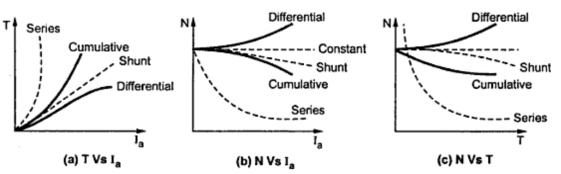
\includegraphics[scale=1]{char.jpeg} 
\caption{Characteristics of DC Motor Field Connections}
\label{fig:1}
\end{figure}

\end{document}